\documentclass[
11pt,%
tightenlines,%
twoside,%
onecolumn,%
nofloats,%
nobibnotes,%
nofootinbib,%
superscriptaddress,%
noshowpacs,%
centertags]%
{revtex4}
\usepackage{ljm}
\usepackage{listings}
\usepackage[utf8]{inputenc}
\usepackage[russian]{babel}

\lstset{
language=C++,
basewidth=0.5em,
xleftmargin=45pt,
xrightmargin=45pt,
basicstyle=\small\ttfamily,
keywordstyle=\bfseries\underbar,
numbers=left,
numberstyle=\tiny,
stepnumber=1,
numbersep=10pt,
showspaces=false,
showstringspaces=false,
showtabs=false,
frame=trBL,
tabsize=2,
captionpos=t,
breaklines=true,
breakatwhitespace=false,
escapeinside={\%*}{*)}
}

\begin{document}

\titlerunning{short name}
\authorrunning{A.~A.~Rybakov and ...}

\title{Title\\Title}

\author{\firstname{A.~A.}~\surname{Rybakov}}
\email[E-mail: ]{rybakov.aax@gmail.com}
\affiliation{Joint Supercomputer Center of the Russian Academy of Sciences -- branch of Scientific Research Institute of System Analysis of the Russian Academy of Sciences, Leninsky prospect 32a, Moscow, 119334, Russia}

\firstcollaboration{(Submitted by S.~S.~Submitter)}

\received{April 01, 2020}

\begin{abstract}
Abstract.
\end{abstract}

\subclass{} % Enter 2010 Mathematics Subject Classification.

\keywords{Keyword1, keyword2.}

\maketitle

\section{Introduction}

Производительность векторного потокового процессора может быть повышена в 5 – 8 раз по сравнению с современными векторными процессорами и почти на два порядка величины – по сравнению с микропроцессорами.

Процессор с архитектурой управления потоком данных (потоковый процессор) имеет потенциал обеспечить наивысшую среди процессоров производительность за счет того, что параллелизм выполнения команд закладывается уже при составлении графа программы, и его не требуется выявлять с помощью сложной аппаратуры из последовательности команд, заданной счетчиком команд, как это имеет место в фон-неймановском процессоре. Программой в потоковых ЭВМ является ориентированный граф, узлами которого являются команды, а информация по дугам передается в виде токенов, содержащих поле данных (значение операнда) и поле контекста передаваемых данных. Этот контекст однозначно определяет, куда должен быть отправлен токен, то есть содержит номер команды приемника в графе программы, а также содержит номера индекса, итерации и запуска подпрограммы, которые позволяют в параллель выполнять различные итерации вложенных циклов и различные запуски процедур на одном и том же графе программы. Причем вне зависимости от места двухвходовой команды в графе она выдаётся на исполнение по прибытию на вход последнего из пары токенов операндов с одинаковым контекстом. После вычисления результата в исполнительном устройстве новые токены со значением результата отправляются на входы последующих команд согласно графу программы, а использованные токены операндов уничтожаются. При этом в потоковом процессоре в отличие от фон-неймановского отсутствует центральное устройство управления (счетчик команд), а параллелизм выполняемых команд определяется в динамике по приходу операндов на входы команд в децентрализованной схеме. А именно, устройство поиска готовых к выполнению команд – память поиска пар (готовых операндов) можно выполнить в виде многих работающих в параллель модулей, обеспечивающих работой такое же большое число исполнительных устройств [1].

Разрабатываемый векторный потоковый процессор (ВПП) имеет наиболее совершенную – динамическую модель потоковой архитектуры, которая позволяет выдавать команды на исполнение по мере готовности их операндов с возможностью одновременного выполнения различных итераций вложенных циклов и различных запусков процедур на одном и том же графе программы. Поиск готовых к выполнению команд в динамических потоковых ЭВМ производится в ассоциативной памяти (АП) по совпадению признаков у токенов операндов, поскольку парные операнды должны иметь не только один и тот же номер выполняемой команды, но и одинаковые поля индекса, номера итерации и запуска процедуры в признаке (контексте) токена. В таких ЭВМ переполнение АП недопустимо, поэтому АП должна иметь большую емкость и в то же время быть быстродействующей, что трудно реализовать на практике.

Введение векторной обработки в динамическую потоковую ЭВМ позволяет существенно снизить требования к емкости АП, поскольку одна векторная команда выполняет не одну, а группу из VL элементарных операций, где VL – длина вектора. При хранении векторов в памяти векторов (ПВ) для выполнения векторной команды требуется поиск в АП лишь одной пары токенов с указателями векторов вместо VL пар токенов при скалярной обработке, и требования к емкости АП на векторизуемой части программы снижаются в VL раз.

В отличие от известных проектов векторных потоковых ЭВМ, в которых арифметические операции над векторами выполняются лишь для векторов в векторных регистрах, в предлагаемом ВПП блок векторных регистров отсутствует и используется одноуровневая ПВ большой емкости (уровня оперативной памяти). При этом исключается проблема возможности переполнения регистрового файла, которая не имеет простого решения, если учесть полную асинхронность потоковой модели вычислений. Так же не просто в процессе выполнения программы обойтись без участия операционной системы при выделении места под создаваемые массивы в основной памяти. Поэтому распределение ресурса ПВ в ВПП предлагается реализовать на аппаратном уровне [2].


\section{Section 1}

Векторный потоковый процессор основан на архитектуре управления потоком данных. Машина с такой архитектурой выдает команды на исполнение по мере готовности их операндов, что позволяет в динамике выявлять и использовать различные виды параллелизма программы. Существует два вида архитектуры управления потоком данных: статическая и динамическая, которая является наиболее совершенной. Динамическая архитектура потокового процессора позволяет одновременно выполнять различные итерации вложенных циклов и различные запуски процедур на одном и том же графе программы. Граф, в свою очередь, является схематичным отображением данных, команд и связей между ними. В каждом узле графа есть какой-либо оператор, а ветви графа указывают на то какие операторы взаимодействуют между собой. В такой архитектуре инструкция начинает выполнятся только тогда, когда данные для нее готовы.

Поиск готовых к выполнению команд в машинах с динамической архитектурой управления потоком данных производится в ассоциативной памяти по совпадению признаков у токенов операндов, так как парные операнды должны иметь не только один и тот же номер выполняемой команды, но и одинаковые поля индекса, номера итерации и запуска процедуры в признаке токена.
Динамическая архитектура имеет более высокую производительность, за счет параллелизма вычислений. Но проблема такой архитектуры заключается в том, что ассоциативная память должна иметь большое пространство для сопоставления всех нужных токенов между собой.
Другой проблемой, стоящей на пути реализации машины с архитектурой управления потоком данных, является проблема организации эффективной работы с массивами данных. Дело в том, что в отличие от фон-неймановской ЭВМ результаты выполняемых команд в исследуемую ЭВМ не записываются в память и не читаются затем из нее в качестве операндов для последующих команд, а, как уже отмечалось ранее, передаются от одной команды к другой в составе токенов согласно графу программы. Причем оба токена операнда после поиска пары и вычисления результата в исполнительном устройстве уничтожаются. Тем самым при выполнении команд работает принцип единственного присваивания, который гарантирует отсутствие последействия, или, так называемых, побочных эффектов. Значит, выдача команды на выполнение определяется лишь наличием операндов на ее входах, и никакие другие условия, например, наличие информации в каких-либо регистрах или ячейках памяти не должны влиять на выдачу команды. Чтобы решить эту проблему, можно внедрить в архитектуру управления потоком данных векторный процессор. Использование векторных команд позволяет в 7 – 10 раз поднять производительность ЭВМ при решении больших научно-технических задач, которые характеризуются обработкой больших массивов данных в 64-разрядном формате чисел с плавающей запятой.

Векторные команды характеризуются тем, что обрабатывают не скалярные значения данных, а векторы – одномерные массивы данных одного и того же формата. Элементами вектора должны быть либо целые числа, либо числа с плавающей запятой, либо битовые значения, над которыми могут выполняться те же основные арифметические и логические операции, что выполняются скалярными командами процессора. Причем векторные команды являются дополнением в системе команд векторной ЭВМ.

Использование векторных команд позволяет векторизовать циклы с отсутствием зависимости по данным между отдельными итерациями. При использовании линейно адресуемой памяти векторов токен может нести в поле данных либо скалярный операнд, либо указатель вектора. В указателе вектора хранится адрес начального элемента вектора в памяти векторов и его фактическая длина. Таким образом для выполнения векторной операции требуется поиск в ассоциативной памяти лишь одной пары токенов с указателями векторов вместо большого количества токенов при скалярной обработке. Следовательно, требования к ассоциативной памяти с точки зрения ёмкости на векторизуемой части программы снижаются в то значение, которому равна длина векторов. В такое же количество раз снижается и число операций для синхронизации обращений к памяти векторов по записи и чтению.

Далее представлена структурная схема векторного потокового процессора.

\begin{figure}[h!]
\setcaptionmargin{5mm}
\onelinecaptionsfalse
\center{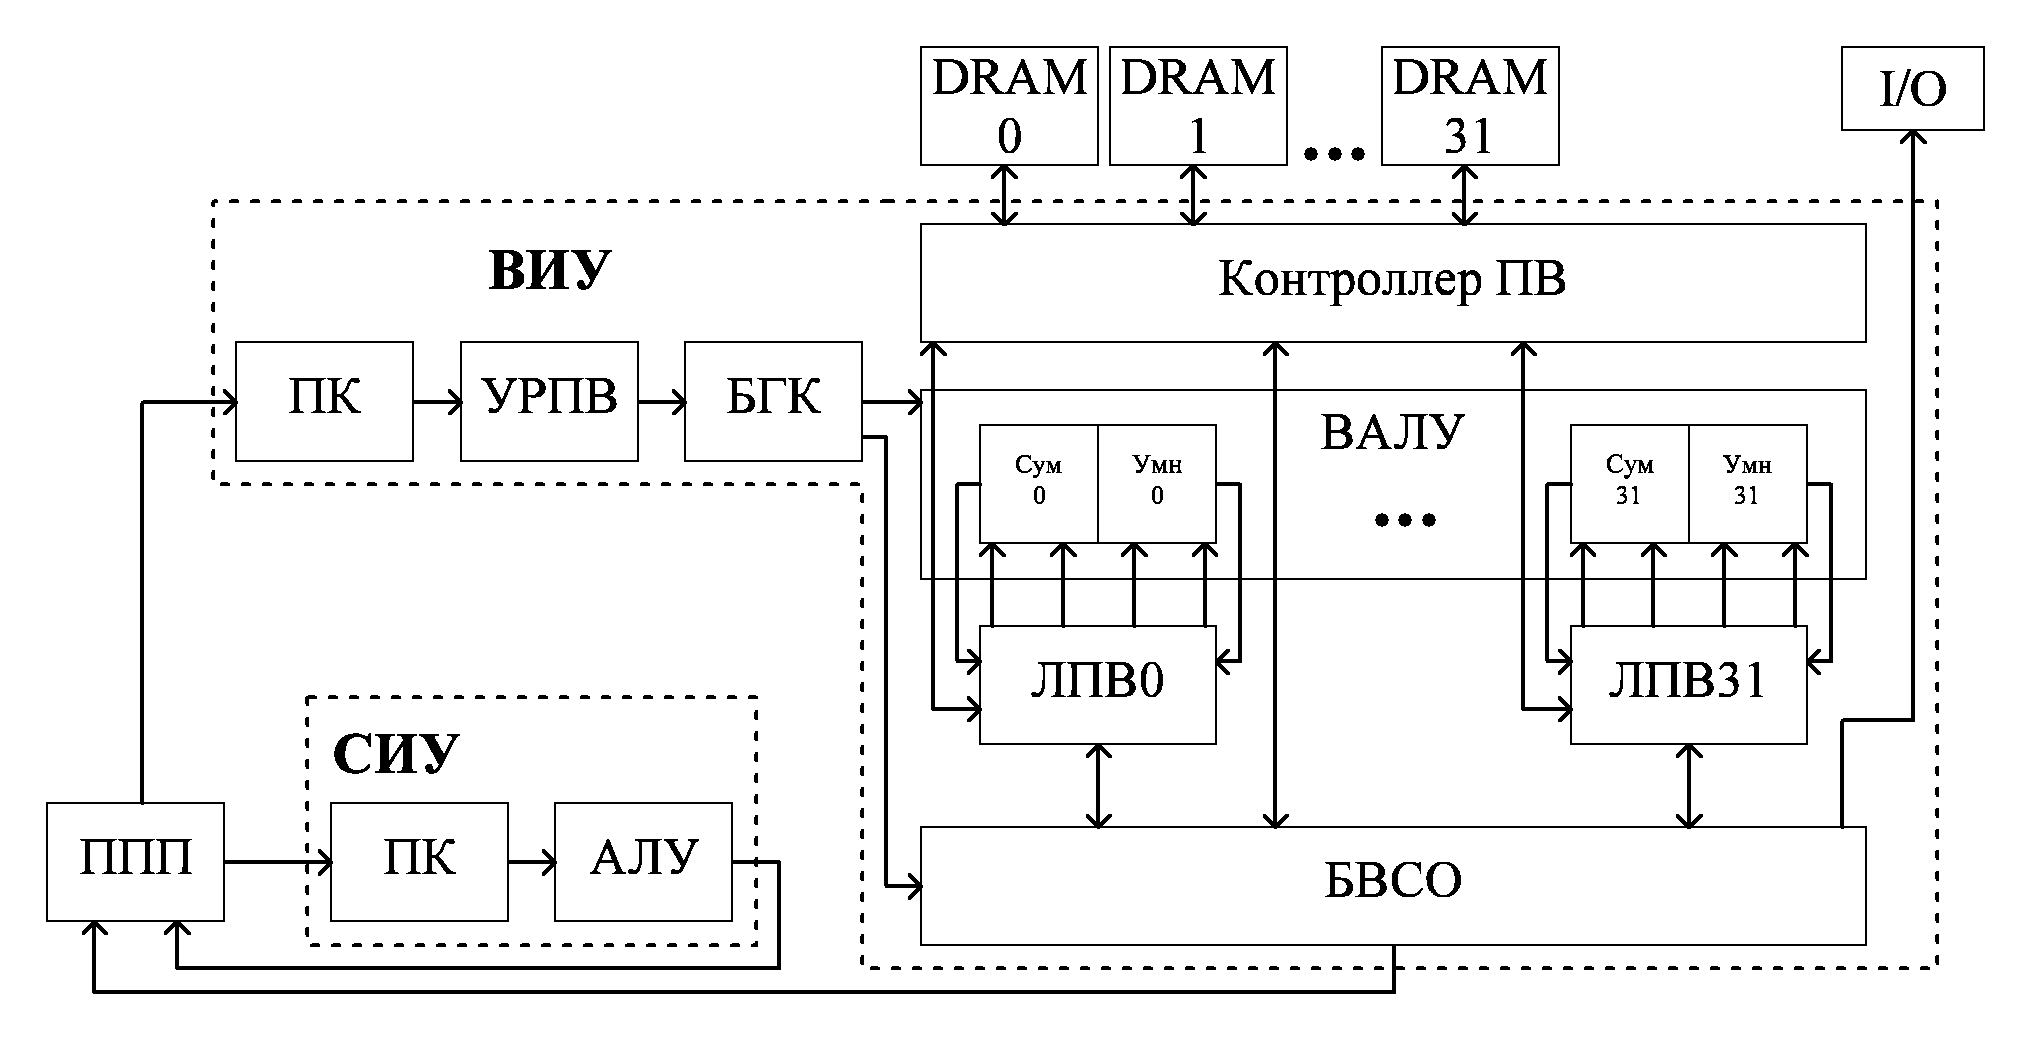
\includegraphics[scale=0.25]{pics/vppschema.png}}
\captionstyle{normal}\caption{Структурная схема векторного потокового процессора}
\label{vpp-scheme}
\end{figure}

Команды, которые готовы для выполнения, из памяти поиска пар (ППП) поступают либо в векторное исполнительное устройство (ВИУ), где выполняются векторные команды, либо в скалярное исполнительное устройство (СИУ), где, соответственно, выполняются скалярные команды. Оба исполнительных устройства конвейерные, в которых на первой ступени конвейера происходит обращение к памяти команд (ПК), откуда по номеру команды в программе выбирается информация, необходимая для выполнения команды в исполнительном устройстве и для формирования токенов результата.
В СИУ после этого происходит вычисление результата в конвейерном арифметико-логическом устройстве (АЛУ) и получившиеся токены со значением результата передаются в ППП для поиска следующих готовых команд.
ВИУ выполняет операции над векторами, элементы которых хранятся в обычной линейно-адресуемой памяти – памяти векторов. Устройство распределения памяти (УРПВ) отводит для каждого результата выполнения векторной команды вектор, который еще не задействован. Адрес начального элемента вектора и его длина являются указателем вектора. Именно этот указатель используется в качестве операнда. Указатель вектора передается из УРПВ в буфер готовых команд (БГК), откуда поступает в ППП, где будет ожидать дальнейшего использования другими командами. Как только все действия с этим вектором были произведены в УРПВ этот вектор поступает в список свободных векторов.
Также на схеме есть локальная память векторов (ЛПВ) и оперативная память, реализованная за пределами кристалла процессора. Локальная и оперативная памяти связаны между собой контроллером памяти векторов (ПВ). Логические операции над элементами векторов производятся в векторном арифметико-логическом устройстве (УРПВ), результат которых переходит в блок выполнения специальных команд (БВСО). 

     
\section{Section 2}

Архитектура эмулятора представляет из себя 4 модуля, которые представлены в виде схеме.

\begin{figure}[h!]
\setcaptionmargin{5mm}
\onelinecaptionsfalse
\center{\includegraphics[scale=0.03]{pics/scheme.pdf}}
\captionstyle{normal}\caption{Comparison of experimental acceleration of a vectorized version of Shell sorting \\ for different sequences of steps.}
\label{shell-sorting-scheme}
\end{figure}

CAM - это модуль, который реализует память поиска пар. Оттуда готовая пара токенов поступает в buffer, который осуществляет промежуточное хранение готовых пар токенов и выдает их на исполнение в память команд - command memory, где выполняются команды.

\section{Conclusion}

Conclusion.

\begin{acknowledgments}
The work has been done at the JSCC RAS as part of the state assignment for the topic ... The supercomputer MVS-10P, located at the JSCC RAS, was used for calculations during the research.
\end{acknowledgments}

\begin{thebibliography}{99}

\bibitem{Rettinger}
\refitem{article}
C. Rettinger, C. Godenschwager, S. Eibl, et al., {\it ``Fully Resolved Simulations of Dune Formation in Riverbeds"}, ISC High Performance , LNCS~{\bf 10266}, 3--21 (2017).

\end{thebibliography}

\end{document}